\chapter{Introdução}
Olá   Mundo!!.
\section{Objetivos}
\begin{enumerate}
	\item Investigar
	\item Obter
\end{enumerate}
Já aprendi um pouco de \LaTeX.
Na verdade, aprendi 10\% de \LaTeX.

Os trabalhos relacionados estão discutidos na seção~\ref{sec:revisao}.
\begin{equation}
	y_{0} = \sum_{i=0}^{N}{x_{i} \times  w_{i}} \times \frac{z}{\alpha}
	\label{eq:teste}
\end{equation}
\section{Revisão da literatura}\label{sec:revisao}
A ativação de um neurônio pode ser descrita pela equação~\ref{eq:ativacao}.
Uma ilustração de um neurônio é apresentada na Figura~\ref{fig:neuronio}.
As notas são apresentadas por meio da Tabela~\ref{tab:tabela}.

O caminho de dados para o processador MIPS contém dois elementos principais~\cite{Hennessy2012}.
Quero citar também~\cite{Staff2018} e  ~\cite{Parham2010}.
\begin{equation}
	y_{0} = \sum_{i=0}^{N}{x_{i} \times  w_{i}} \times \frac{z}{\alpha}
	\label{eq:ativacao}
\end{equation}

\begin{figure}[htb]
	\centering
	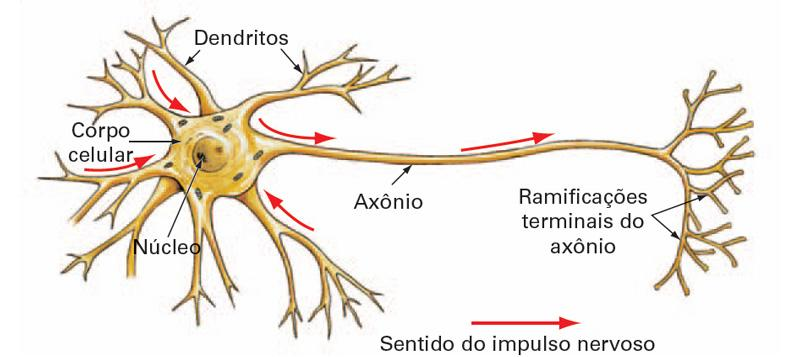
\includegraphics[scale=.3]{neuronio}
	\caption{Neurônio artificial}
	\label{fig:neuronio}
\end{figure}


\begin{table}[htb]
	\centering
	\caption{Teste de Tabela}
	\begin{tabular}{ccr}
		\hline
		\textbf{RA} & \textbf{Nome} & 
		\textbf{Nota} \\
		\hline
		2323 & Luciano & 8,0 \\
		3232 & Jose & 7,0 \\
		\hline
	\end{tabular}
	\label{tab:tabela}
\end{table}
\lstset{language=C}
\begin{lstlisting}[frame=single, numbers=left]
	int a = 5;
	void main(){
		if( a > 5 ){
			printf( "Hello World\n");
		}
	}
	
	
	
\end{lstlisting}
\lstinputlisting[frame=single, numbers=left]{exemplo.py}

\lipsum[3-8]
%\bibliographystyle{plain}
